% =====================================================================
%  ORB — PROJECT REPORT
%  Department of Computer Science, CHRIST (Deemed to be University)
%  Format: CHRIST Project Report Guidelines
%    - A4, one-side; Left 1.5in, Right 1in, Top 1in, Bottom 1in
%    - Times New Roman; Chapter titles 16pt bold caps centered;
%      side headings 12pt bold caps; body 12pt; 1.5 line spacing
%    - Header: project name (left) + page number (right), 10pt, ruled
%    - Footer: department name, 10pt, ruled
%    - Roman page numbers from Acknowledgements; Arabic from Chapter 1
%    - No header/footer/page number on Title page, Certificate, TOC
%  Compile: pdflatex (run twice for TOC/cross-references)
% =====================================================================
\documentclass[12pt,a4paper,oneside]{report}

% ---------- Fonts: Times New Roman equivalent ----------
\usepackage[T1]{fontenc}
\usepackage[utf8]{inputenc}
\usepackage{newtxtext,newtxmath}   % Times-compatible text + math
\usepackage[htt]{hyphenat}         % allow hyphenation inside \texttt paths
\usepackage{microtype}             % character protrusion: cleaner justification
\emergencystretch=1.5em            % avoid overfull lines in narrow columns

% ---------- Page geometry ----------
\usepackage[a4paper,
    left=1in, right=1in, top=1in, bottom=1in]{geometry}

% ---------- Line spacing ----------
\usepackage{setspace}
\setstretch{1.5}

% ---------- Graphics, tables, misc ----------
\usepackage{graphicx}
\usepackage{ragged2e}
\usepackage{xcolor}
\usepackage{etoolbox}
\graphicspath{{../architecture/images/}{../../images/}{./images/}}
\usepackage{array}
\usepackage{longtable}
\usepackage{booktabs}
\renewcommand{\arraystretch}{1.25}   % breathing room in table rows
\usepackage{enumitem}
\setlist{itemsep=2pt,topsep=4pt}
\usepackage{url}
\urlstyle{same}                      % URLs in Times, not typewriter
\usepackage[hidelinks]{hyperref}

% ---------- Captions: 10pt; figure caption below, table caption above ----------
\usepackage{caption}
\captionsetup{font=small,labelfont=bf,labelsep=space,justification=centering}
\captionsetup[table]{position=above,skip=6pt}
\captionsetup[figure]{position=below,skip=6pt}
\renewcommand{\figurename}{Fig}
\renewcommand{\tablename}{Table}
% Thin border for UI screenshots so they separate from the page
\newcommand{\screenshot}[2][0.9\textwidth]{%
  \setlength{\fboxsep}{0pt}\setlength{\fboxrule}{0.4pt}%
  \fbox{\includegraphics[width=#1]{#2}}}

% ---------- Chapter / section heading styles ----------
\usepackage{titlesec}
% Chapter: 16pt bold, capital letters, centered
\titleformat{\chapter}[block]
  {\centering\normalfont\fontsize{16}{19}\selectfont\bfseries}
  {\MakeUppercase{\chaptertitlename}\ \thechapter :}
  {0.5em}
  {\MakeUppercase}
\titlespacing*{\chapter}{0pt}{-10pt}{20pt}
% Section (side heading): 12pt bold, capital letters
\titleformat{\section}
  {\normalfont\fontsize{12}{14.4}\selectfont\bfseries}
  {\thesection}{0.6em}{\MakeUppercase}
\titlespacing*{\section}{0pt}{14pt}{6pt}
% Subsection: 12pt bold, capital letters
\titleformat{\subsection}
  {\normalfont\fontsize{12}{14.4}\selectfont\bfseries}
  {\thesubsection}{0.6em}{}
\titlespacing*{\subsection}{0pt}{12pt}{4pt}

% ---------- Header and footer ----------
\usepackage{fancyhdr}
\definecolor{darkred}{RGB}{139,0,0}
\newcommand{\ProjectName}{Orb}
\newcommand{\DeptFooter}{Department of Computer Science, CHRIST (Deemed to be University)}
% \patchcmd{\headrule}/\patchcmd{\footrule} must run exactly ONCE, here in
% the preamble. \fancypagestyle{...}{...} bodies are re-executed on every
% single page that uses the style, so patching \headrule/\footrule from
% inside a style body re-patches an already-patched macro on the second such
% page onward; etoolbox's internal scratch definition (\etb@resrvda) then
% gets typeset as literal text instead of drawing a rule. Patch once here;
% the style bodies below only ever set widths (idempotent, safe every page).
\patchcmd{\headrule}{\hrule}{\color{darkred}\hrule}{}{}
\patchcmd{\footrule}{\hrule}{\color{darkred}\hrule}{}{}
\fancypagestyle{orbmain}{%
  \fancyhf{}%
  \fancyhead[L]{\small\textbf{\ProjectName}}%
  \fancyhead[R]{\small\thepage}%
  \fancyfoot[L]{\small \DeptFooter}%
  \renewcommand{\headrulewidth}{0.8pt}%
  \renewcommand{\footrulewidth}{0.8pt}%
}
% Chapter-opening pages use the same header/footer
\fancypagestyle{plain}{%
  \fancyhf{}%
  \fancyhead[L]{\small\textbf{\ProjectName}}%
  \fancyhead[R]{\small\thepage}%
  \fancyfoot[L]{\small \DeptFooter}%
  \renewcommand{\headrulewidth}{0.8pt}%
  \renewcommand{\footrulewidth}{0.8pt}%
}
% Front pages with no header/footer (Title page, Certificate)
\fancypagestyle{blankstyle}{%
  \fancyhf{}%
  \renewcommand{\headrulewidth}{0pt}%
  \renewcommand{\footrulewidth}{0pt}%
}

% ---------- Widow/orphan control (do not end a page with a heading
%            or a single first line of a paragraph) ----------
\clubpenalty=10000
\widowpenalty=10000
\displaywidowpenalty=10000
\raggedbottom
% Float-only pages: content starts at the top, not vertically centered
\makeatletter
\setlength{\@fptop}{0pt}
\setlength{\@fpbot}{0pt plus 1fil}
\makeatother

% =====================================================================
\begin{document}
\normalfont
\fontsize{12}{18}\selectfont

% =====================================================================
%  FRONT MATTER OMITTED FOR NOW
%  Title Page, Certificate, AI Usage Declaration Statement,
%  Acknowledgement and Abstract are individually signed per student and
%  submitted separately (Orb_Report_Front5_<Name>.tex/pdf, generated by
%  make_front5.py from an earlier, already-approved revision of this
%  file). They are intentionally NOT regenerated here so this build
%  cannot drift from the three already-signed copies; they will be
%  merged back into this file once signed. Do not re-add that content
%  by hand — regenerate the Front5 copies from this file only after the
%  next signing round.
% =====================================================================

% ---------------- TABLE OF CONTENTS / LIST OF FIGURES / LIST OF TABLES ----------------
\pagenumbering{roman}
\setcounter{page}{1}
\pagestyle{plain}
\begin{singlespace}
\renewcommand{\contentsname}{Table of Contents}
\tableofcontents
\clearpage
\renewcommand{\listfigurename}{List of Figures}
\listoffigures
\addcontentsline{toc}{chapter}{List of Figures}
\clearpage
\renewcommand{\listtablename}{List of Tables}
\listoftables
\addcontentsline{toc}{chapter}{List of Tables}
\clearpage
\end{singlespace}

% =====================================================================
%  MAIN MATTER — Arabic numbering starts at Chapter 1
% =====================================================================
\pagenumbering{arabic}
\setcounter{page}{1}
\pagestyle{orbmain}

% =====================================================================
\chapter{Introduction}
% =====================================================================

\section{Overview}
Language models have moved from remote, provider-hosted services to
software that runs directly on personal computers. Runtimes such as
Ollama make it possible to serve models like Qwen~3 and Gemma~3 on a
laptop, while cloud providers such as Anthropic, OpenAI, Groq and
Mistral expose increasingly capable models through public APIs. In
both cases, modern usage goes beyond plain text generation: models are
given \emph{tools} --- the ability to read and write files, execute
shell commands and search the web --- and are run in an agentic loop
where the model decides which tool to call next.

This shift creates a governance problem. A model that can execute
\texttt{bash} commands or read arbitrary files on the host machine is
effectively an autonomous actor on that machine, yet common chat
interfaces provide no policy layer, no audit trail and no measure of
how trustworthy a given answer is. \textbf{Orb} is our response to
this problem: a web-based governance console that sits between the
user and the model. All inference --- local or cloud --- passes
through a governed gateway that enforces execution policy on every
tool call, records detailed audit logs, tracks latency and token
telemetry, scores responses for hallucination risk, and maintains
long-term, per-user memory, all behind authenticated access.

\section{Problem Statement}
Existing interfaces to local and cloud language models suffer from the
following gaps:
\begin{itemize}
  \item \textbf{No execution governance.} When a model requests a tool
        action (file read, file write, shell command, web search),
        interfaces either execute it silently or refuse it entirely;
        there is no per-tool policy of allow, block or
        require-human-approval.
  \item \textbf{No auditability.} There is no durable record of what
        was asked, which tools ran, what they returned and what policy
        decisions were taken --- a prerequisite for any responsible
        deployment.
  \item \textbf{No trust signal.} Users receive fluent answers with no
        indication of how likely the response is to be fabricated.
  \item \textbf{Fragmented provider access.} Local models and each
        cloud provider come with separate interfaces, credentials and
        conventions; there is no single governed entry point.
  \item \textbf{No durable context.} Facts a user states in one
        conversation are forgotten in the next unless the user repeats
        them.
\end{itemize}
The problem, therefore, is to design and implement a single oversight
layer that provides policy enforcement, auditing, telemetry,
risk scoring and memory across heterogeneous model backends.

\section{Objectives of the Project}
\begin{itemize}
  \item To build a unified, authenticated web console from which a
        user can converse with local Ollama models and cloud models
        (Anthropic, OpenAI, Groq, Mistral) through one governed
        gateway.
  \item To enforce a per-tool execution policy --- Auto, Policy or
        Manual approval --- on every tool call made by a model, with
        the ability to pause an agent run until a human approves.
  \item To provide a programmatic, Bearer-token API
        (\texttt{/api/v1/*}) whose every call is written to an audit
        log with request messages, tool calls, tool results, policy
        decisions, latency and token counts.
  \item To compute a hallucination-risk score for each response and
        expose per-session telemetry (latency, first-token time,
        blocked actions).
  \item To extract durable user facts from conversations into a
        per-user memory store that is automatically injected into
        future system prompts.
  \item To manage provider credentials centrally through a connectors
        module in which database-stored keys override environment
        variables.
  \item To persist sessions so that conversations can be listed,
        inspected and resumed with their full message history,
        policies and settings.
  \item To let an administrator upload a company AI-usage policy
        document, have it compiled by a language model into
        structured, reviewable rules, and --- once activated ---
        enforce those rules for every user and API key ahead of the
        existing per-session policy.
\end{itemize}

\section{Scope of the Project}
Orb targets a single-machine, local-first deployment: the gateway,
database and frontend run on the user's computer, and local inference
never leaves the machine. The system supports five provider
connectors (Anthropic, OpenAI, Groq, Mistral for chat; Google for key
storage), four governed tools (file-system read, file write, shell
execution, web search via Tavily), interactive use through a browser
and programmatic use through API keys. It supports one company-wide
policy document at a time, compiled into action rules (enforced at
the tool gate) and conduct rules (injected into the system prompt and
checked by the post-chat judge); per-department or per-team policy
scoping is out of scope for the present iteration. Multi-node deployment,
fine-tuning of models, and enforcement \emph{inside} the model runtime
are outside the present scope and are discussed as future
enhancements in Chapter~8.

\section{Organisation of the Report}
Chapter~2 analyses the existing systems and establishes feasibility.
Chapter~3 specifies functional, non-functional, hardware and software
requirements. Chapter~4 presents the system design --- architecture,
data-flow diagrams, database schema and sequence flows. Chapter~5
describes the implementation of each module. Chapter~6 covers the
testing strategy and test cases. Chapter~7 presents the results with
screenshots of the working system. Chapter~8 concludes the report and
lists future enhancements, followed by references and appendices.

% =====================================================================
\chapter{System Analysis}
% =====================================================================

\section{Existing System}
Interaction with language models today occurs mainly through three
kinds of software. Provider web chat applications (e.g., provider
consoles for GPT or Claude) are polished but cloud-only: every prompt
leaves the user's machine, no local models can be used, and the user
has no control over tool execution policy. Local runtimes such as
Ollama expose a REST endpoint on \texttt{localhost:11434} and simple
CLI chat, but offer no authentication, no persistence beyond the
terminal, no policy layer and no telemetry. General-purpose LLM
front-ends add chat history on top of local runtimes but treat the
model as a text generator only --- when tool use is supported at all,
it is executed without per-tool governance, and none of them produce
an audit trail suitable for review.

\subsection{Limitations of the Existing System}
\begin{itemize}
  \item Tool calls (shell, file access, web) execute without a policy
        gate or human-approval checkpoint.
  \item No unified interface spans both local models and multiple
        cloud providers with centrally managed credentials.
  \item No audit log records requests, tool activity and decisions.
  \item No indicator of response reliability is shown to the user.
  \item Conversations are either lost or stored without any associated
        telemetry, and facts about the user are not carried forward.
\end{itemize}

\section{Proposed System}
The proposed system, Orb, is a governance console composed of a
Next.js frontend and an Express/TypeScript gateway backed by SQLite.
All model traffic flows through the gateway, which adds six
capabilities missing from existing systems: (i)~a policy engine that
resolves every tool call to \emph{Allowed}, \emph{Blocked} or
\emph{Requires Approval}, pausing the agent loop for manual approval;
(ii)~full audit logging of programmatic API traffic; (iii)~telemetry
--- per-message latency, first-token time and a hallucination-risk
index computed asynchronously after each reply; (iv)~per-user memory
extraction so that durable facts are injected into future prompts;
(v)~a connectors module that stores provider API keys in the
database, overriding environment variables, so that local and cloud
models are reached through one interface; and (vi)~a company policy
document pipeline that compiles an uploaded AI-usage policy into
structured rules with a human review-and-activate step, then layers
those rules --- most-restrictive-wins --- over the existing per-session
policy for every user and API key.

\subsection{Advantages of the Proposed System}
\begin{itemize}
  \item Human-in-the-loop control over dangerous operations such as
        shell execution and file writes.
  \item Complete, queryable audit history for programmatic access.
  \item A trust signal (risk score) attached to responses.
  \item Single governed entry point for five providers plus local
        inference, with API keys managed centrally.
  \item Organisation-wide rules from a single uploaded policy document,
        enforced automatically without every user hand-configuring
        per-tool rules.
  \item Local-first privacy: local inference and all governance data
        remain on the user's machine.
\end{itemize}

\section{Feasibility Study}

\subsection{Technical Feasibility}
The system is built entirely from mature, freely available
technologies: Node.js with Express and TypeScript for the gateway,
Next.js with React for the frontend, SQLite (via
\texttt{better-sqlite3}) for storage, Clerk for identity, and Ollama
for local inference. All components run on commodity hardware; local
models such as Qwen~3 and Gemma~3 run acceptably on a machine with
8--16~GB of RAM, and the gateway itself is lightweight. No component
requires specialised infrastructure, so the project is technically
feasible.

\subsection{Economic Feasibility}
Every framework and library used is open source and free of licence
cost. Local inference through Ollama incurs no per-token charges;
cloud providers are optional and pay-as-you-go, with keys supplied by
the user. Development required only the team's existing laptops.
The project is therefore economically feasible for an academic
setting.

\subsection{Operational Feasibility}
The console runs in a standard web browser with a familiar chat
interface, so no special training is needed for basic use. Policy
configuration and API-key management are presented through dedicated
screens with sensible defaults (safe tools auto-allowed, dangerous
tools requiring approval). Because the system is self-hosted and
local-first, it fits environments where data cannot leave the
machine, which widens rather than narrows its operational
applicability.

% =====================================================================
\chapter{System Requirements Specification}
% =====================================================================

\section{Functional Requirements}
\begin{itemize}
  \item \textbf{FR-1 Authentication.} The system shall authenticate
        interactive users via Clerk session cookies and programmatic
        clients via \texttt{orb\_sk\_...} Bearer API keys verified by
        SHA-256 hash lookup.
  \item \textbf{FR-2 Chat.} The system shall stream chat responses as
        NDJSON from local Ollama models or cloud providers selected by
        the user, within an agentic loop that supports tool calls.
  \item \textbf{FR-3 Policy enforcement.} The system shall support
        three chat modes --- \emph{Auto} (all tools allowed),
        \emph{Manual} (every tool call requires approval) and
        \emph{Policy} (per-tool rules of Allowed / Blocked / Requires
        Approval) --- and shall pause the loop, emitting a
        \texttt{requires\_approval} event, when approval is needed;
        approved calls resume via a dedicated endpoint. Blocked calls
        shall be reported back to the model as refusals. Where an
        active company policy document applies, its decision for a
        tool call shall be merged with the session-level decision by
        taking the more restrictive of the two.
  \item \textbf{FR-4 Tool execution.} The system shall provide
        governed tools for file read, file write, directory listing,
        shell execution and Tavily web search.
  \item \textbf{FR-5 Sessions.} The system shall persist every
        conversation with its messages, policies and settings; users
        shall be able to list, inspect, complete and resume sessions.
  \item \textbf{FR-6 Memory.} The system shall asynchronously extract
        durable user facts after each exchange, store them per user,
        inject them into future system prompts, and allow the user to
        view and delete them.
  \item \textbf{FR-7 Risk scoring.} The system shall compute a
        hallucination-risk score for each assistant reply and attach
        it to the persisted message.
  \item \textbf{FR-8 API keys and audit.} The system shall create,
        list, revoke and re-scope API keys with per-key tool flags
        (\texttt{fs}, \texttt{bash}, \texttt{web}), and shall write an
        audit row for every \texttt{/api/v1/chat} call containing
        request messages, response, tool calls/results, policy
        decisions, latency, token counts and status code.
  \item \textbf{FR-9 Analytics.} The system shall summarise audit
        activity (volume, blocked and error counts, latency, hourly
        buckets, top tools, anomalies) over a selectable window.
  \item \textbf{FR-10 Connectors.} The system shall store provider API
        keys for Anthropic, OpenAI, Groq, Mistral and Google, mask
        them on read, and resolve keys with database values overriding
        environment variables.
  \item \textbf{FR-11 Model discovery.} The system shall list locally
        installed Ollama models and detect host CPU/RAM to recommend a
        performance mode.
  \item \textbf{FR-12 Policy document compilation.} The system shall
        accept an uploaded policy document (PDF, DOCX, Markdown, TXT
        or a pre-compiled JSON rule set), extract its text, and
        compile it in the background into \emph{action} rules
        (tool, matched field, match kind, pattern, effect) and
        \emph{conduct} rules (a plain-language directive), each
        retaining the source excerpt it was derived from; the
        resulting rule set shall remain in \emph{review} and shall
        not be enforced until an administrator activates it.
  \item \textbf{FR-13 Policy document lifecycle and enforcement.} The
        system shall let an administrator review, edit, enable or
        disable, and activate exactly one company policy document at
        a time; while active, its enabled action rules shall be
        evaluated against every tool call ahead of the session-level
        policy (most restrictive wins), its enabled conduct rules
        shall be injected into the system prompt and checked by the
        post-chat judge, a \emph{monitor} mode shall allow rules to be
        logged without being enforced, and every decision (allowed,
        blocked, approval required, approved, denied, monitored,
        flagged) shall be recorded with its triggering rule for audit.
\end{itemize}

\section{Non-Functional Requirements}
\begin{itemize}
  \item \textbf{NFR-1 Privacy.} Local inference and all governance
        data (sessions, memories, audit logs, keys) shall remain on
        the user's machine in a local SQLite file.
  \item \textbf{NFR-2 Responsiveness.} Responses shall be streamed
        token-by-token; first-token time and total latency shall be
        measured and displayed.
  \item \textbf{NFR-3 Security.} API keys shall be stored only as
        SHA-256 hashes with last-four digits for display; provider
        keys shall be masked whenever read back; dangerous tools shall
        default to manual approval; policy document upload, editing
        and activation shall be restricted to an administrator
        allow-list when one is configured, and open to any signed-in
        user otherwise; regular-expression rule patterns shall be
        validated against catastrophic backtracking before they are
        stored.
  \item \textbf{NFR-4 Reliability.} The database shall run in WAL mode;
        post-chat analysis shall be fire-and-forget so that a failure
        in analysis never breaks the chat path.
  \item \textbf{NFR-5 Usability.} All governance features shall be
        reachable from a single-page console with dedicated screens
        for chat, sessions, memory, API keys and connectors.
  \item \textbf{NFR-6 Maintainability.} The backend shall be written
        in typed TypeScript with modular routes, repositories and a
        provider-agnostic LLM interface so that new providers can be
        added by implementing one class.
\end{itemize}

\section{Hardware Requirements}
\begin{table}[h]
\caption{Hardware requirements}
\centering
\begin{tabular}{p{4.5cm}p{8.5cm}}
\toprule
\textbf{Component} & \textbf{Minimum specification} \\
\midrule
Processor & 64-bit quad-core CPU (Apple Silicon / Intel i5 or better) \\
RAM & 8 GB (16 GB recommended for larger local models) \\
Storage & 20 GB free (local model weights are 2--8 GB each) \\
Display & Any modern display; browser-based UI \\
Network & Required only for cloud providers, Clerk and web search \\
\bottomrule
\end{tabular}
\end{table}

\section{Software Requirements}
\begin{table}[h]
\caption{Software requirements}
\centering
\begin{tabular}{p{4.5cm}p{8.5cm}}
\toprule
\textbf{Category} & \textbf{Software} \\
\midrule
Operating system & macOS / Linux / Windows \\
Runtime & Node.js 20+ \\
Backend & Express 4, TypeScript, tsx; \texttt{better-sqlite3} 13 \\
Frontend & Next.js 16 (App Router), React 19, Framer Motion, GSAP \\
Database & SQLite (WAL mode), file \texttt{backend/data/orb.db} \\
Authentication & Clerk (\texttt{@clerk/nextjs}, \texttt{@clerk/express}) \\
Local inference & Ollama (models: Qwen 3, Gemma 3) \\
Cloud SDKs & \texttt{@anthropic-ai/sdk}; OpenAI-compatible HTTP for
             OpenAI / Groq / Mistral \\
Web search & Tavily (\texttt{@tavily/core}) \\
Tools & Git, VS Code, npm \\
\bottomrule
\end{tabular}
\end{table}

\section{Technologies Used}

\subsection{Next.js and React}
The frontend is a single-page Next.js App-Router application. React 19
renders the console's screens (landing, chat, sessions, memory, API,
connectors), while Framer Motion and GSAP provide the animated
transitions. The frontend communicates with the gateway over
\texttt{fetch} with credentials included, consuming NDJSON streams for
chat.

\subsection{Express and TypeScript}
The gateway is an Express 4 application written in TypeScript and run
with \texttt{tsx}. Routes are grouped by resource (chat, sessions,
memories, keys, connectors, models, system) with two authentication
middlewares: \texttt{requireAuth} (Clerk cookie) for interactive
routes and \texttt{apiKeyAuth} (Bearer hash lookup) for
\texttt{/api/v1/*}.

\subsection{SQLite with better-sqlite3}
Storage is a single SQLite file opened in WAL mode through the
synchronous \texttt{better-sqlite3} driver --- an appropriate choice
for a single-writer, local-first application. Structured values
(messages, settings, policies, tool flags) are stored as JSON columns,
a deliberate denormalisation for low-concurrency local use.

\subsection{Clerk}
Clerk is the external identity provider: sign-in and sign-up pages are
Clerk components in the frontend, and the backend verifies session
cookies via \texttt{@clerk/express}. There is no local users table;
\texttt{user\_id} columns hold Clerk user IDs.

\subsection{Ollama and Cloud Providers}
Local inference uses Ollama's streaming chat API on
\texttt{localhost:11434}. Cloud inference is abstracted behind a
common \texttt{LLM} interface with three implementations: Ollama,
Anthropic (official SDK) and an OpenAI-compatible client reused for
OpenAI, Groq and Mistral. A factory selects the implementation from
the chosen model and resolves the provider key through the connectors
module.

% =====================================================================
\chapter{System Design}
% =====================================================================

\section{Architecture Overview}
Orb follows a three-tier, gateway-centred architecture. The
presentation tier is the Next.js console; the application tier is the
Express gateway containing authentication, the agent loop, the policy
engine, tool executor, connectors resolver and post-chat analysis; the
data tier is SQLite. External actors are the browser user
(Clerk-authenticated), third-party API clients (key-authenticated),
Clerk, local Ollama, the four cloud chat providers and the Tavily
search API. The defining property of the architecture is that
\emph{no model call and no tool call can bypass the gateway}: policy,
audit and telemetry are applied at the single choke point through
which all traffic flows.

\section{Data Flow Diagrams}

\subsection{Context Level (Level 0)}
Fig~4.1 shows the system as a single process exchanging data with six
external entities and one data store. Users and third-party clients
send chat, session, key, memory and connector requests; the platform
verifies identities with Clerk, performs completions against Ollama or
cloud providers, issues search queries to Tavily, and reads and writes
all five tables of \texttt{orb.db}.

\begin{figure}[h]
\centering
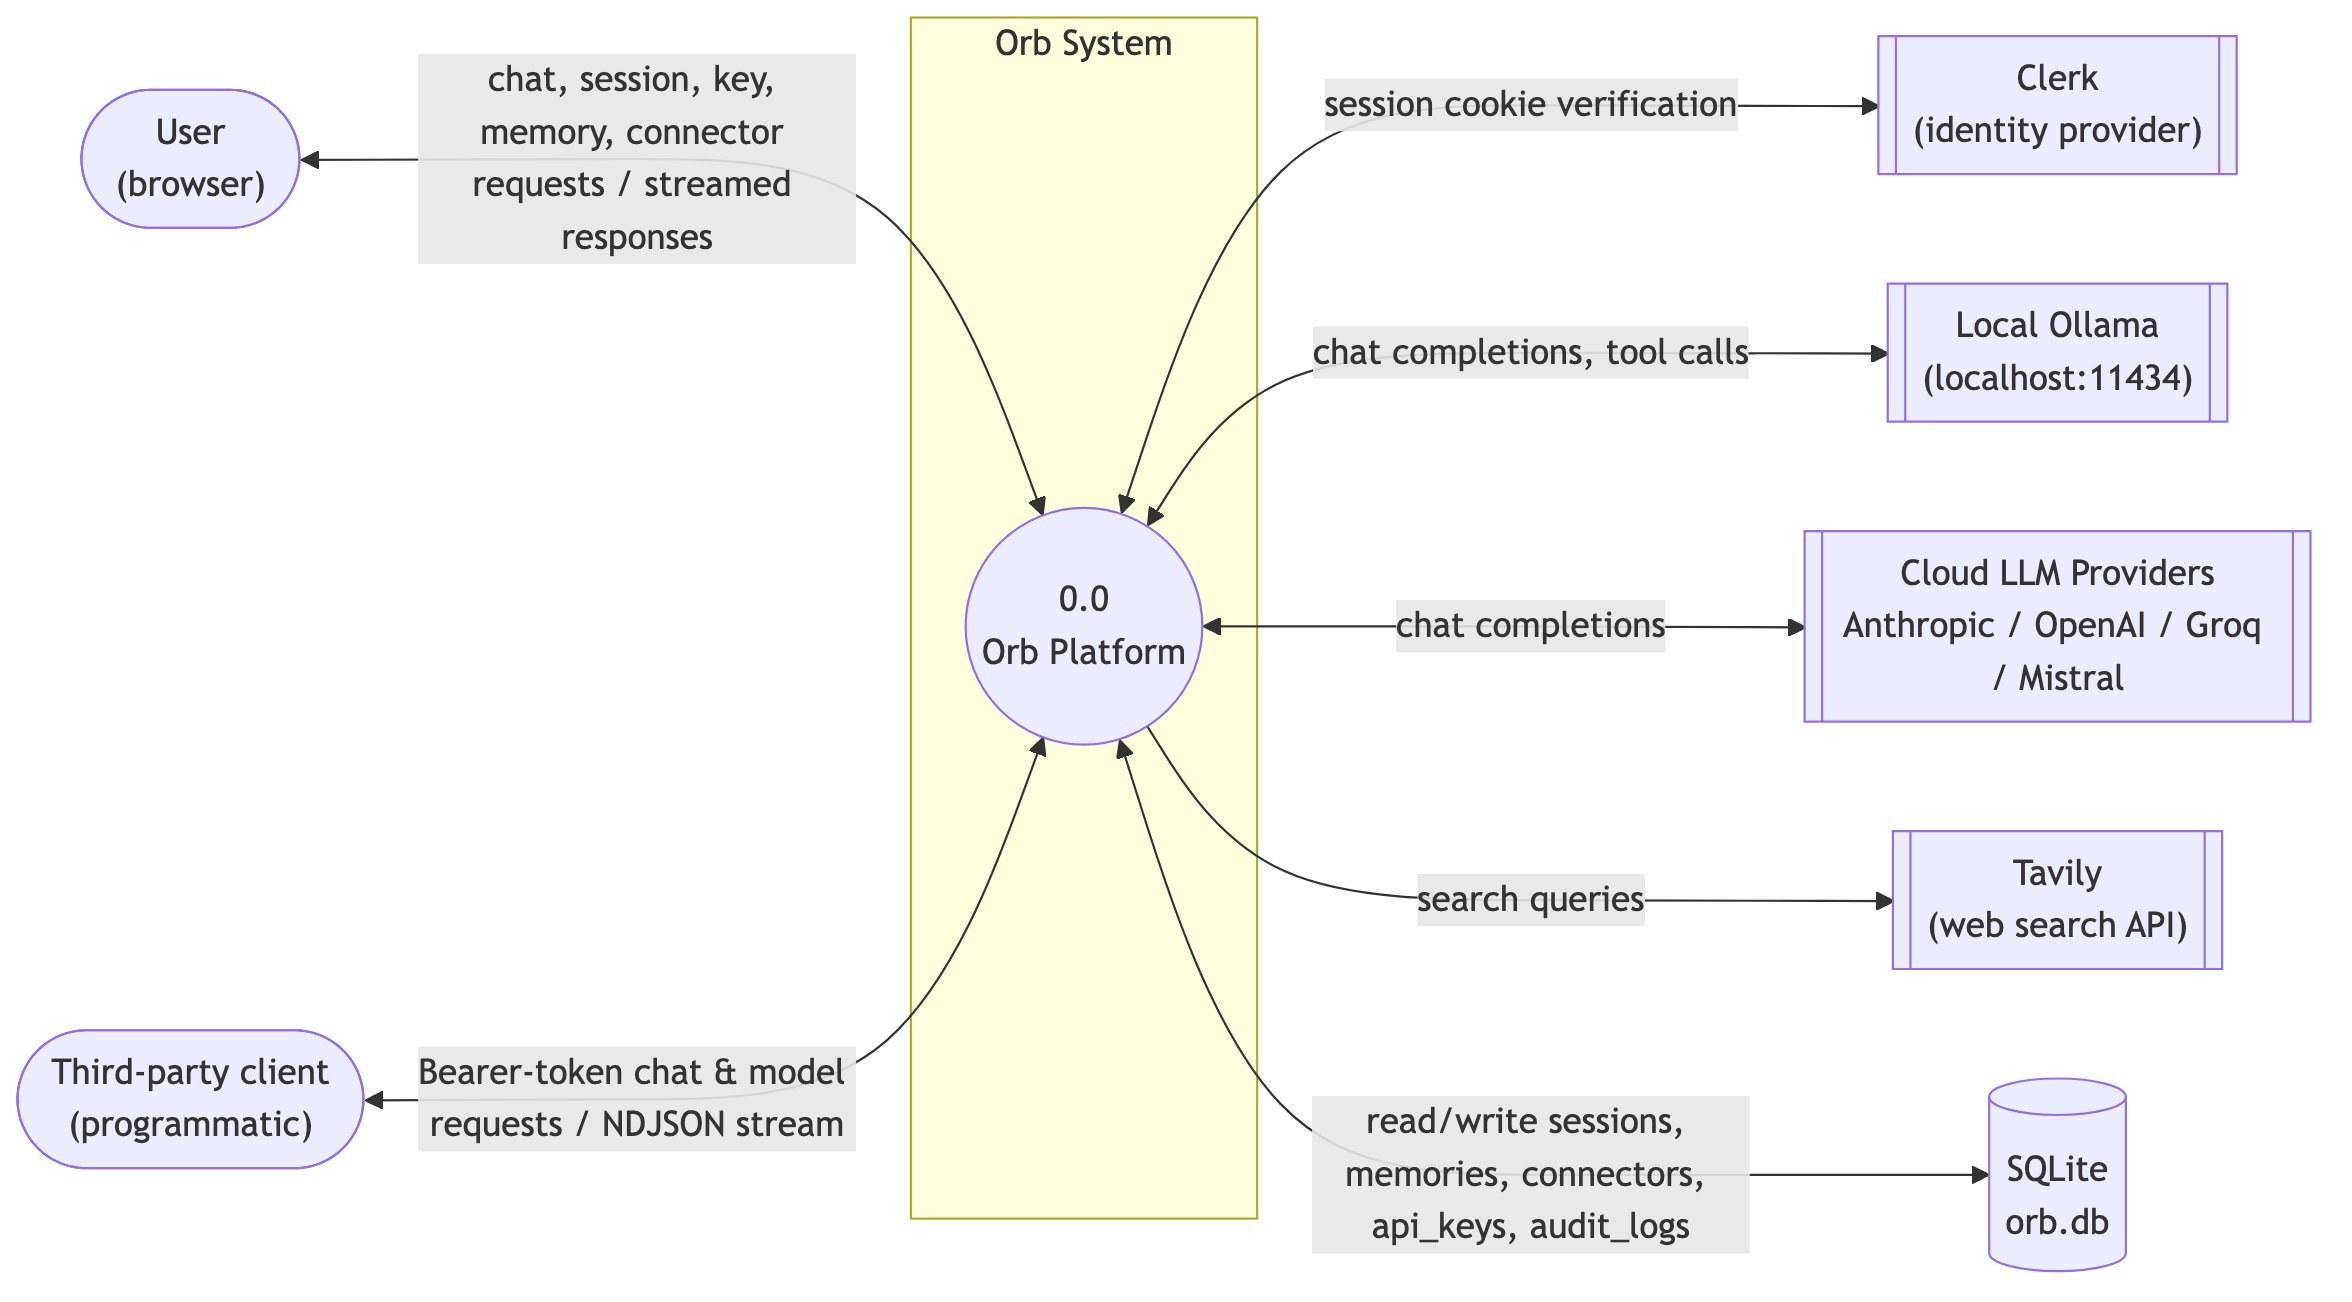
\includegraphics[width=0.95\textwidth]{context-dfd.png}
\caption{Context-level data flow diagram}
\end{figure}

\subsection{Level 1 Decomposition}
At Level 1 the platform decomposes into nine processes:
authentication (1.0), session management (2.0), the agent loop (3.0),
tool execution (4.0), connector key resolution (5.0), memory
extraction and risk scoring (6.0), API-key and audit management
(7.0), connector management (8.0) and memory management (9.0). The
agent loop is the hub: it loads sessions and memories, resolves
provider keys, dispatches allowed tool calls, streams to the client,
fires post-chat analysis asynchronously and, for programmatic calls,
logs to the audit store.
% Export the Level 1 DFD PNG from docs/architecture/dfd.md (Mermaid source)
% and place it as level1-dfd.png, then uncomment:
% \begin{figure}[h]
% \centering
% \includegraphics[width=0.95\textwidth]{level1-dfd.png}
% \caption{Level 1 data flow diagram}
% \end{figure}

\section{Database Design}
The schema (Fig~4.2) has eight tables. Clerk is the source of truth
for identity, so there is no local users table; \texttt{user\_id}
columns are logical references to Clerk IDs. Two foreign keys are
enforced: \texttt{audit\_logs.api\_key\_id} $\rightarrow$
\texttt{api\_keys(id)} and \texttt{policy\_rules.document\_id}
$\rightarrow$ \texttt{policy\_documents(id)}; the reference columns on
\texttt{policy\_events} are deliberately logical (unenforced) so that
audit rows outlive an edited or deleted rule or document.

\begin{figure}[h]
\centering
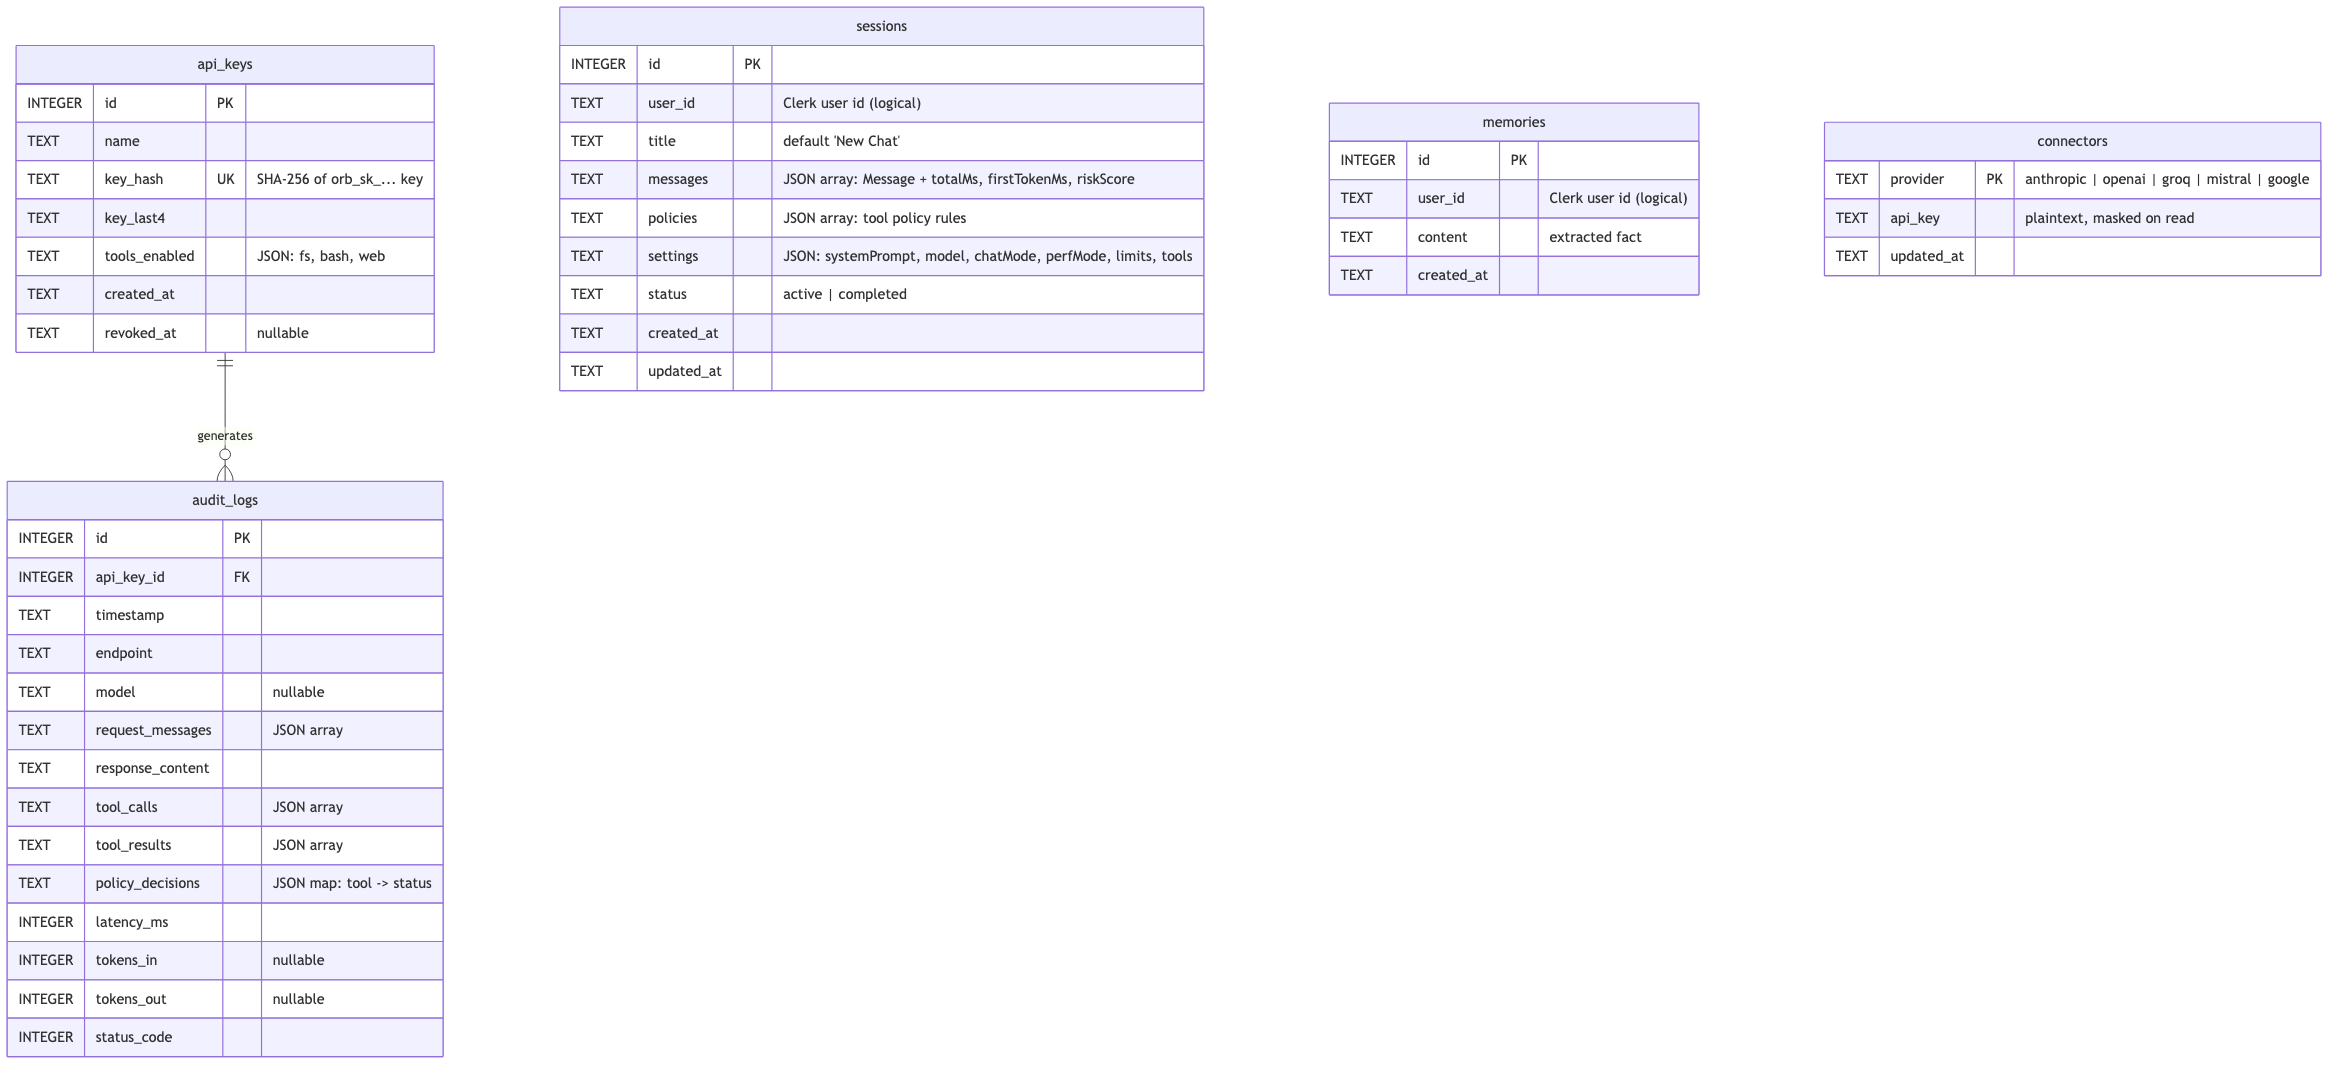
\includegraphics[width=0.9\textwidth]{erd.png}
\caption{Entity--relationship diagram}
\end{figure}

\begin{table}[h]
\caption{Database tables and their purpose}
\centering
\begin{tabular}{p{3cm}p{10cm}}
\toprule
\textbf{Table} & \textbf{Purpose} \\
\midrule
\texttt{sessions} & One row per conversation: title, JSON message
array (with per-message latency, first-token time and risk score),
JSON policy rules, JSON settings (system prompt, model, chat mode,
performance mode, limits, tools), status (active/completed). \\
\texttt{memories} & Durable facts extracted per user; injected into
future system prompts. \\
\texttt{connectors} & One row per provider (\texttt{anthropic},
\texttt{openai}, \texttt{groq}, \texttt{mistral}, \texttt{google});
stores the provider API key, upserted on save, masked on read. \\
\texttt{api\_keys} & Programmatic credentials: name, SHA-256 hash,
last four characters, JSON tool flags (\texttt{fs}, \texttt{bash},
\texttt{web}), revocation timestamp. \\
\texttt{audit\_logs} & One row per \texttt{/api/v1/chat} call:
endpoint, model, request messages, response content, tool calls and
results, per-tool policy decisions, latency, token counts, status
code. \\
\texttt{policy\_documents} & One row per uploaded policy document:
title, filename, extracted source text, lifecycle status
(compiling/review/active/archived/failed), enforcement mode
(enforce/monitor), compile model, compile notes/errors, uploader. \\
\texttt{policy\_rules} & Rules compiled (or manually added) for a
policy document: kind (action/conduct), title, effect
(allow/deny/require\_approval/advise), for action rules the tool,
matched field, match kind and pattern, for conduct rules the
directive text, the source excerpt it was derived from, origin
(compiled/manual) and an enabled flag. \\
\texttt{policy\_events} & One row per policy decision: timestamp,
channel (chat/api/execute\_tool/executor/judge/dry\_run), tool,
truncated arguments, decision (allowed/blocked/approval\_required/
approved/denied/monitored/flagged), source and the triggering
document/rule, for audit and the Policies screen's events feed. \\
\bottomrule
\end{tabular}
\end{table}

\section{Process Design: The Agent Loop}
An interactive chat request follows the sequence: the frontend posts
to \texttt{/api/chat}; \texttt{requireAuth} verifies the Clerk cookie;
the route loads or creates the active session and reads the user's
memory facts; a system prompt is assembled from the facts and the
tool-use directive; the LLM factory instantiates the correct provider
client (resolving connector keys for cloud models); and the agent loop
streams model output in a reason--act--observe cycle. Whenever the
model emits a tool call, the policy resolver classifies it according
to the session's chat mode --- \emph{Auto} allows all tools,
\emph{Manual} holds every call, and \emph{Policy} applies per-tool
rules: \emph{Allowed} calls are executed by the ToolExecutor and
their results fed back into the loop; \emph{Blocked} calls are
injected back as refusal messages so the model can continue; and
\emph{Requires Approval} pauses the loop and emits a
\texttt{requires\_approval} event, after which the frontend can invoke
\texttt{/api/execute\_tool} to resume. After the final reply, the
route persists messages with timing data and fires
\texttt{postChatAnalysis} asynchronously, which extracts new facts
into \texttt{memories} and patches the message's risk score.

The programmatic path (\texttt{/api/v1/chat}) differs in three ways:
authentication is by hashed Bearer key; the allowed tool set is
derived from the key's \texttt{tools\_enabled} flags rather than
session policies; and every call is written to \texttt{audit\_logs}.

\section{Company Policy Document Pipeline}
An administrator uploads a policy document on the Policies
screen; the gateway extracts its text (\texttt{pdf-parse} for PDF,
\texttt{mammoth} for DOCX, verbatim for Markdown/TXT, or a
pre-compiled rule array for JSON) and stores the document with status
\emph{compiling}. A background job chunks the text on paragraph
boundaries, prompts the selected model per chunk to extract
\emph{action} rules (tool, matched field, match kind, pattern,
effect) and \emph{conduct} rules (a plain-language directive), each
quoting the source sentence it came from, validates and deduplicates
the result, and moves the document to \emph{review}. Validation
rejects a rule whose field is incompatible with its tool, whose
pattern is missing where required, or whose regular expression fails
an \texttt{safe-regex2} catastrophic-backtracking check. Nothing is
enforced in this state: the administrator inspects, edits, enables,
disables or manually adds rules, then \emph{activates} the document,
which atomically archives whichever document was previously active.

Once active, every tool call is evaluated against the document's
enabled action rules --- \emph{deny} beats \emph{require\_approval}
beats \emph{allow} beats no match --- and the result is merged with
the existing session-level decision (chat mode or, for a key, its
tool scope) by taking whichever of the two is more restrictive; a
document \emph{require\_approval} that reaches the key-authenticated
API, where no human can approve it, degrades to \emph{blocked}.
Setting the document to \emph{monitor} mode computes the same
decision but never enforces it, logging it instead so an
administrator can observe impact before enforcing. Enabled conduct
rules are appended to every system prompt, and the same post-chat
judge that scores hallucination risk is asked which conduct rules, if
any, the reply violated; violations are attached to the message and
shown in the console, but never block a reply. The tool executor also
carries its own hard-deny check against the active document, so a
denied action cannot run even if a caller reached it by a path other
than the policy resolver. Every decision --- blocked, approval
required, approved, denied, monitored or flagged --- is written to
\texttt{policy\_events} with its triggering document and rule.
% TODO: add a Policies-screen screenshot to images/ (e.g. 06_policies.png)
% and reinstate a \screenshot figure here once one has been captured.

\section{Connector Key Resolution}
Cloud provider credentials are resolved by a two-level lookup
(Fig~4.3): the factory first queries the \texttt{connectors} table;
if no row exists it falls back to the corresponding
\texttt{<PROVIDER>\_API\_KEY} environment variable. Database values
therefore override environment configuration, allowing keys to be
managed from the console at runtime without restarting the server.

\begin{figure}[h]
\centering
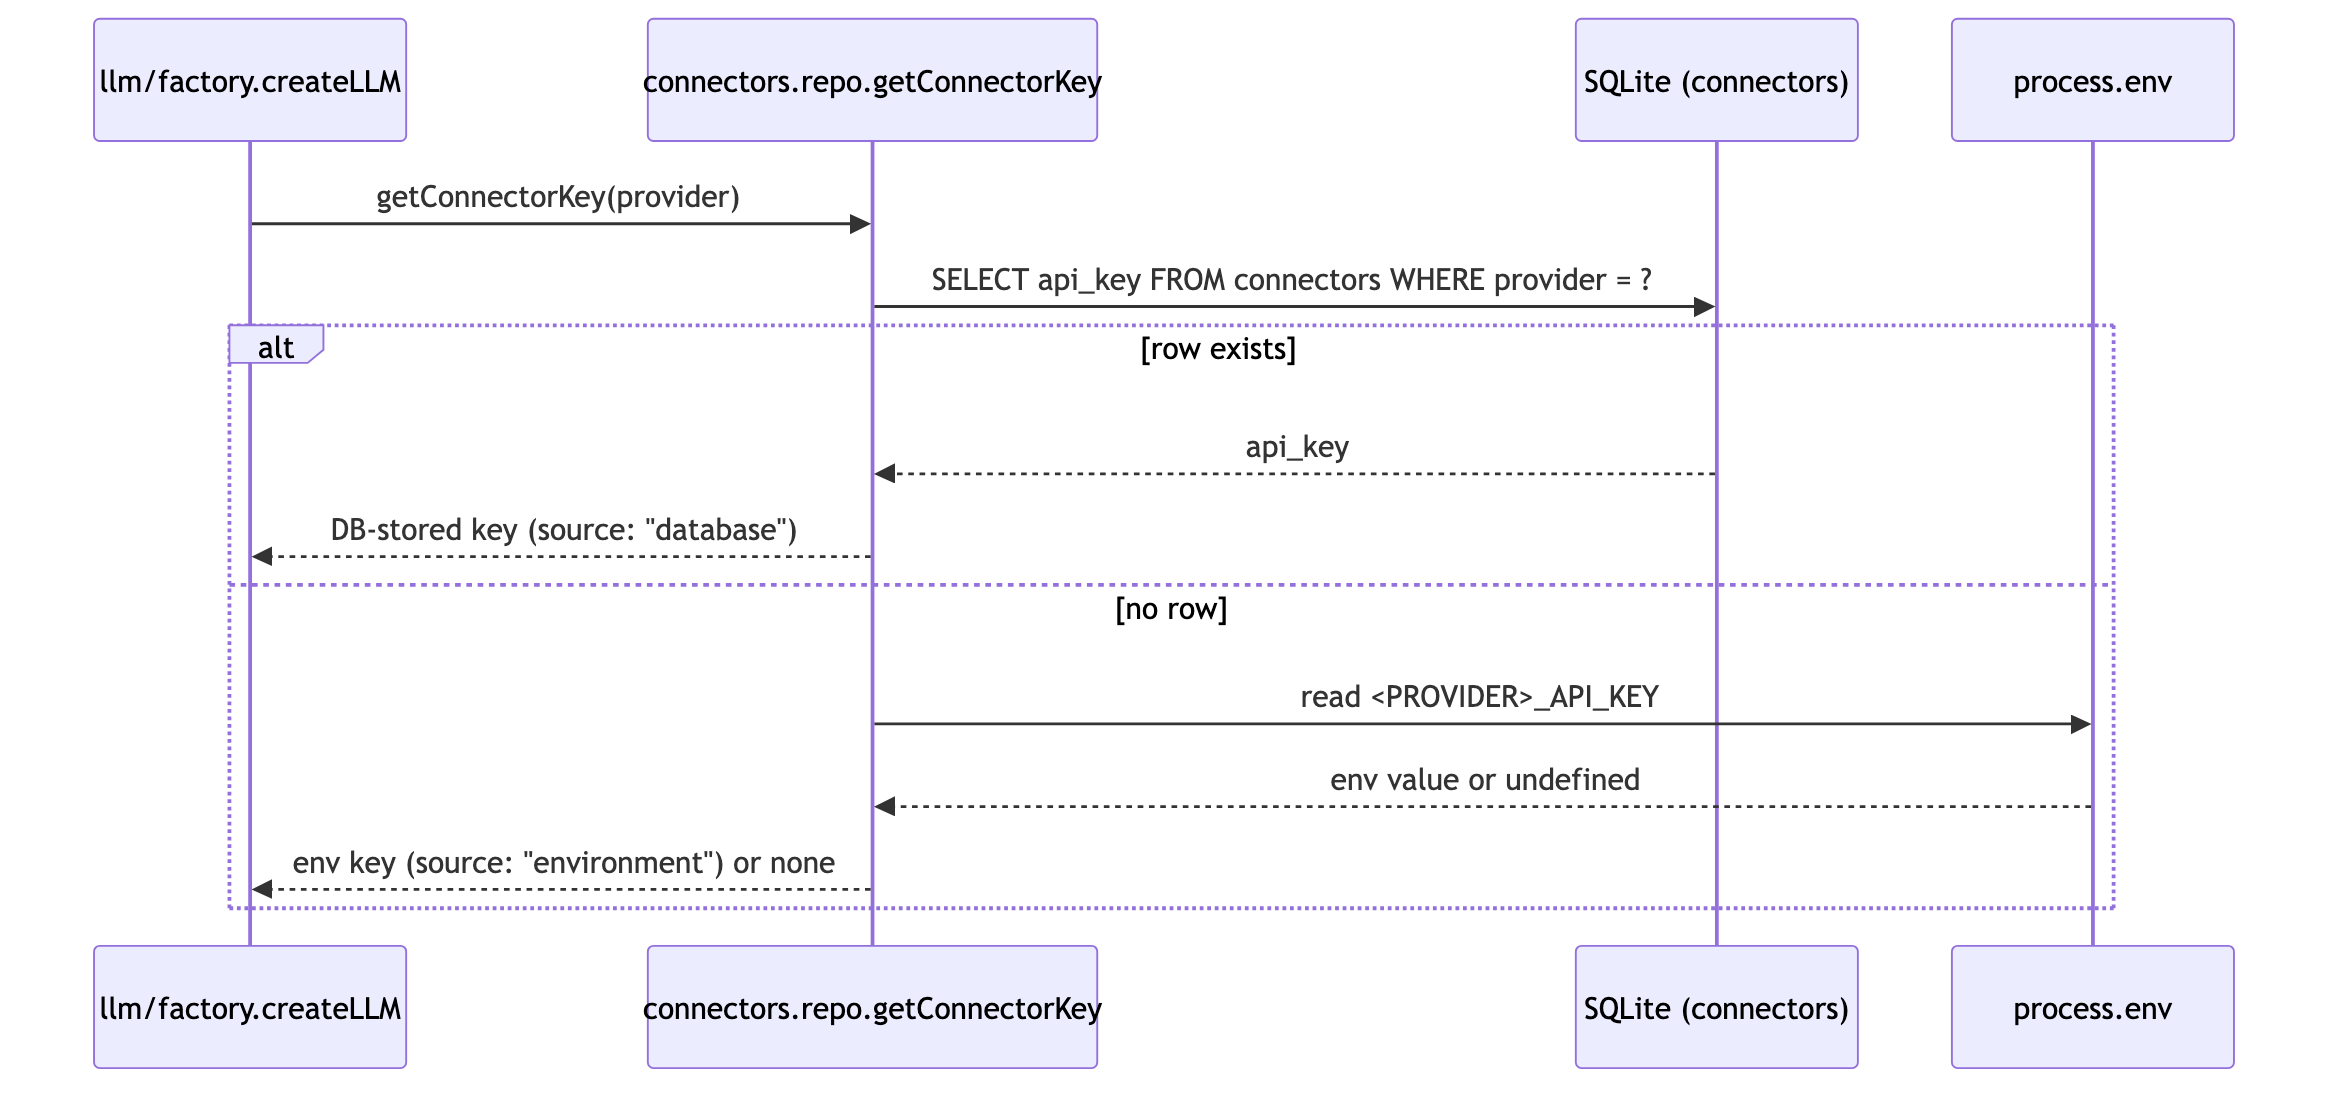
\includegraphics[width=0.75\textwidth]{seq-connector-resolution.png}
\caption{Connector key resolution sequence}
\end{figure}

\section{API Design}
The gateway exposes two authentication surfaces: cookie-authenticated
interactive routes and key-authenticated programmatic routes.
Table~4.2 summarises the main endpoints.

\begin{table}[h]
\caption{Principal API endpoints}
\centering
\begin{singlespace}
\footnotesize
\begin{tabular}{p{2.1cm}p{5.2cm}p{1.5cm}p{4.2cm}}
\toprule
\textbf{Method} & \textbf{Path} & \textbf{Auth} & \textbf{Purpose} \\
\midrule
POST & \texttt{/api/chat} & cookie & Stream agent run (NDJSON) \\
POST & \texttt{/api/execute\_tool} & cookie & Resume after approval \\
POST & \texttt{/api/v1/chat} & API key & Programmatic agent run,
audited \\
GET & \texttt{/api/models} & none & List local Ollama models \\
GET & \texttt{/api/system-info} & none & CPU/RAM detection \\
GET/PATCH & \texttt{/api/sessions/active} & cookie & Active session,
policy/settings patch \\
GET & \texttt{/api/sessions[/:id]} & cookie & List / inspect
sessions \\
POST & \texttt{/api/sessions/:id/resume} & cookie & Reactivate a
session \\
GET/DELETE & \texttt{/api/memories[/:id]} & cookie & List / delete
facts \\
POST/GET & \texttt{/api/keys} & cookie & Create / list API keys \\
DEL / PATCH & \texttt{/api/keys/:id[...]} & cookie & Revoke /
re-scope key \\
GET & \texttt{/api/audit-logs} & cookie & Recent audit rows \\
GET & \texttt{/api/analytics/summary} & cookie & Usage analytics \\
GET/POST & \texttt{/api/connectors} & cookie & List / save provider
keys \\
DELETE & \texttt{/api/connectors/:provider} & cookie & Remove stored
key \\
POST & \texttt{/api/policies/upload} & cookie, admin & Upload a policy
document; compilation runs in the background \\
GET & \texttt{/api/policies[/:id]} & cookie & List documents / inspect
one with its rules \\
POST & \texttt{/api/policies/:id/activate} & cookie, admin & Archive
the current active document and activate this one \\
POST/PATCH/ DELETE & \texttt{/api/policies/:id/rules[/:ruleId]} &
cookie, admin & Add, edit, enable/disable or delete a rule \\
POST & \texttt{/api/policies/evaluate} & cookie & Dry-run a tool call
against the active document without persisting a decision \\
GET & \texttt{/api/policies/events}, \texttt{/stats} & cookie & Recent
policy decisions / counts by outcome \\
\bottomrule
\end{tabular}
\end{singlespace}
\end{table}
Mutating policy endpoints additionally require the caller to be in an
optional administrator allow-list (\texttt{POLICY\_ADMIN\_USER\_IDS});
when the list is unset, every signed-in user may manage policies.

\section{User Interface Design}
The console is a single-page application with screen-level navigation:
a cinematic \emph{Landing} screen, the \emph{App} (chat) screen with
model selector, chat modes (Ask / Search / Research), policy controls
and live telemetry, a \emph{Sessions} screen listing past
conversations with average latency, risk and policy-flag counts, a
\emph{Memory} screen for viewing and deleting extracted facts, an
\emph{API} screen for key management, audit logs and analytics, a
\emph{Connectors} screen listing all five providers with configuration
state and masked keys, and a \emph{Policies} screen for uploading a
policy document, watching it compile, reviewing and editing the
extracted rules grouped by kind, activating or archiving the document,
toggling enforce/monitor mode, dry-running a tool call against the
active policy, and inspecting recent policy decisions. On the chat
screen, a blocked action renders as a red card naming the triggering
rule and its source (company policy, chat mode or session policy), an
approval prompt names the company-policy rule that required it when
applicable, and a flagged reply shows which conduct rule the post-chat
judge believes it violated. Sign-in and sign-up are Clerk-hosted
components. The UI uses vanilla CSS variables for light/dark theming.

% =====================================================================
\chapter{Implementation}
% =====================================================================

\section{Implementation Environment}
The system is organised as two Node.js applications in one repository:
\texttt{backend/} (Express + TypeScript gateway, run with
\texttt{tsx}, listening on port 3001) and \texttt{frontend/} (Next.js
console on port 3000). SQLite storage is created on first start by
\path{backend/src/db/init.ts} using idempotent \texttt{CREATE TABLE
IF NOT EXISTS} statements. Development followed an iterative,
feature-branch workflow with Git.

\section{Module Description}

\subsection{Authentication Module}
Two middlewares guard the gateway. \texttt{requireAuth} validates the
Clerk session cookie on all interactive \texttt{/api/*} routes and
attaches the Clerk \texttt{userId} to the request.
\texttt{apiKeyAuth} handles \texttt{/api/v1/*}: it hashes the
presented \texttt{orb\_sk\_...} token with SHA-256, looks up
\texttt{api\_keys.key\_hash}, rejects revoked keys and attaches the
key row (including its \texttt{tools\_enabled} flags) to the request.
Plaintext keys are shown exactly once at creation; only the hash and
last four characters are stored.

\subsection{LLM Abstraction and Factory}
All providers implement a common \texttt{LLM} interface
(\texttt{backend/src/llm/LLM.ts}) exposing a streaming chat method.
\texttt{Ollama.ts} adapts the local runtime;
\texttt{Anthropic.ts} wraps the official SDK; and
\texttt{OpenAICompatible.ts} is a single client parameterised by base
URL, reused for OpenAI, Groq and Mistral. \texttt{factory.ts}
dispatches by model-name prefix (\texttt{claude-} $\rightarrow$
Anthropic, \texttt{gpt-} $\rightarrow$ OpenAI, \texttt{groq/}
$\rightarrow$ Groq, \texttt{mistral/} $\rightarrow$ Mistral, anything
else $\rightarrow$ local Ollama), applies performance-mode parameters
(context size, prediction limits, history trimming, keep-alive) and
resolves cloud credentials via the connectors repository.

\subsection{Agent Loop and Policy Engine}
\texttt{Agent.ts} implements the reason--act--observe loop: stream
model output; forward content chunks to the client; on a tool call,
ask the policy resolver for a status; loop with tool results until
the model replies without tool calls. Interactive runs resolve policy
from the session's chat mode (\texttt{chatMode.ts}): \emph{Auto}
allows every tool, \emph{Manual} pauses on every call with a
\texttt{requires\_approval} event until the user approves via
\texttt{/api/execute\_tool}, and \emph{Policy} applies per-tool rules
(Allowed / Blocked / Requires Approval) configured in the console.
Blocked calls are injected back into the conversation as refusal
messages so the model can adapt, and are surfaced in telemetry as
blocked actions. Programmatic runs derive the allowed set from the
API key's tool flags instead. When a company policy document is
active, the resolver evaluates it as a second, independent layer and
merges the two decisions by taking whichever is more restrictive, so
\texttt{Agent.ts} itself stays unaware of where a decision came from
--- it only ever sees a single \texttt{Allowed}/\texttt{Blocked}/
\texttt{Requires Approval} status with an attached reason.

\subsection{Tool Executor}
\texttt{ToolExecutor.ts} dispatches approved calls to the registered
tools: \texttt{FsTool} (read file), \texttt{WriteFileTool},
\texttt{ListDirectoryTool}, \texttt{BashTool} (shell execution) and
\texttt{WebSearchTool} (Tavily). Each tool validates its arguments and
returns a structured result that is appended to the conversation and
streamed to the client as \texttt{tool\_call\_intent} and
\texttt{tool\_result} events.

\subsection{Policy Document Module}
The \texttt{backend/src/policy/} package is organised so the
decision logic is independent of the database: \texttt{matcher.ts}
implements the five match kinds (\texttt{any}, \texttt{contains},
\texttt{prefix}, \texttt{glob} with \texttt{picomatch}, \texttt{regex}
guarded by \texttt{safe-regex2}), normalising and expanding
\texttt{\textasciitilde} in path arguments before comparison;
\texttt{evaluate.ts} is a pure function that merges a document
decision with a session decision and applies monitor-mode and
API-degradation rules, with no database access, so it can be exercised
directly by an automated test harness; \texttt{engine.ts} caches the
active document and its enabled rules in memory, invalidated on every
write, and exposes the tool executor's hard-deny check;
\texttt{resolver.ts} wraps the engine for \texttt{Agent.ts}, logging
one \texttt{policy\_events} row per decision; \texttt{extractText.ts}
and \texttt{compiler.ts} extract and chunk the document and drive the
LLM extraction prompt, validating and deduplicating the rules it
returns; and \texttt{prompt.ts} renders the active conduct and
deny/approval rules as a bounded ``Company policy'' section appended
to every system prompt. \texttt{db/policies.repo.ts} and
\texttt{api/policies.route.ts} follow the same repository/route
pattern as the rest of the gateway.

\subsection{Session Management Module}
\texttt{sessions.route.ts} maintains one active session per user with
endpoints to read and patch its policies and settings, complete it
(``New Chat''), list all sessions with computed average latency and
risk, inspect any session and resume a completed one. Messages are
persisted with per-message \texttt{totalMs}, \texttt{firstTokenMs} and
\texttt{riskScore}.

\subsection{Memory and Risk Analysis Module}
After each interactive reply, \texttt{postChatAnalysis.ts} runs
asynchronously: it sends the exchange to a local Ollama model
(with thinking disabled and unbounded prediction for reliable JSON
extraction from thinking models such as Qwen~3) and receives new user
facts and a hallucination-risk value. Facts are inserted into
\texttt{memories}; the risk score is patched onto the persisted
message. When a company policy is active, the same call also asks the
model which of the active conduct rules, if any, the reply violated;
matched rule ids are attached to the message as advisory policy flags
and logged to \texttt{policy\_events}, never blocking the reply.
Because the call is fire-and-forget, analysis failures never affect
the chat path.

\subsection{Connectors Module}
\texttt{connectors.route.ts} and \texttt{connectors.repo.ts} manage
provider keys for the five known providers. Keys are upserted per
provider, masked on every read, and deletable (falling back to
environment variables). Resolution order --- database first, then
environment --- lets the console override server configuration at
runtime.

\subsection{API Keys, Audit and Analytics Module}
\texttt{keys.route.ts} creates keys with per-key tool scopes, lists
them masked, revokes and re-scopes them. Every \texttt{/api/v1/chat}
call is written by the audit repository with the complete request and
response payloads, tool activity, per-tool policy decisions, latency,
token counts and status code. The analytics endpoint aggregates this
log into volume, blocked/error counts, latency statistics, hourly
buckets, top tools and anomalies over a selectable window.

\subsection{Frontend Console}
The console (\texttt{frontend/src/app/page.tsx}) implements
screen-level navigation between Landing, Transition, App (chat),
Sessions, Memory, API, Connectors and Policies screens. The chat
screen consumes the NDJSON stream incrementally, renders markdown with
syntax highlighting, surfaces tool-call intents and approval prompts
inline, and displays live telemetry. The Policies screen uploads a
document by \texttt{FormData} (the JSON body size limit does not apply
to file uploads), polls the document while it compiles, and lets an
administrator review, edit and activate its rules. Framer Motion and
GSAP drive the animated transitions; Clerk components provide sign-in
and sign-up.

% =====================================================================
\chapter{Testing}
% =====================================================================

\section{Testing Strategy}
Testing combined three approaches. First, manual functional testing
against the running system: each functional requirement of Chapter~3
was exercised through the console. Second, API-level verification
using \texttt{curl} for the programmatic routes, with Bearer keys of
varying scopes. Third, an automated model-behaviour evaluation
harness (\path{backend/scripts/eval-tool-calls.ts}) that runs five
tool-calling scenarios against a live Ollama model --- imperative
shell requests, question-phrased shell, web-search and file-read
requests, and a pure-knowledge question expected to trigger \emph{no}
tool call --- reporting pass/fail per case. A second, dependency-free
harness (\path{backend/scripts/eval-policy-engine.ts}) unit-tests the
policy engine directly: rule matching for each of the five match
kinds including \texttt{\textasciitilde}-expansion for glob patterns,
the deny/require\_approval/allow precedence within a document,
most-restrictive-wins merging against a session decision in both
directions, monitor mode never blocking, the API's
require\_approval-to-blocked degradation, and rule validation
including regex-safety rejection --- 49 assertions, all passing. It
was run against a realistic sample policy
(\path{backend/scripts/sample-policy.md}) compiled end-to-end with a
local Qwen~3 model, which correctly extracted eleven rules (six
action, five conduct) and produced the expected decision for nine
representative tool calls. Emphasis throughout was
placed on the policy engine (the security-critical path),
authentication boundaries and the resilience of the asynchronous
analysis stage. Formal unit and integration test suites beyond these
two harnesses are an acknowledged gap, noted as future work.

\section{Test Cases}
Table~6.1 lists representative test cases covering authentication,
policy enforcement, connector resolution, memory extraction and
failure handling, together with the observed outcomes.
\begin{table}[!t]
\caption{Representative test cases}
\centering
\begin{singlespace}
\footnotesize
\setlength{\tabcolsep}{4pt}
\begin{tabular}{p{1.1cm}p{4.1cm}p{4.0cm}p{2.5cm}p{1.2cm}}
\toprule
\textbf{ID} & \textbf{Scenario} & \textbf{Expected result} &
\textbf{Actual result} & \textbf{Status} \\
\midrule
TC-01 & Unauthenticated call to \texttt{/api/sessions} & 401 rejected
& As expected & Pass \\
TC-02 & Chat with local Qwen 3 model & Streamed NDJSON reply, message
persisted with latency & As expected & Pass \\
TC-03 & Model requests \texttt{bash} under Manual policy & Loop pauses
with \texttt{requires\_approval}; resumes after approval & As expected
& Pass \\
TC-04 & Model requests blocked tool & Call blocked, decision recorded,
loop continues & As expected & Pass \\
TC-05 & \texttt{/api/v1/chat} with key lacking \texttt{bash} scope &
Bash tool unavailable to model; audit row written & As expected &
Pass \\
TC-06 & Revoked API key used & 401 rejected & As expected & Pass \\
TC-07 & Save Anthropic key in Connectors, then chat with Claude &
DB key used (source ``database''), chat succeeds & As expected &
Pass \\
TC-08 & Delete stored key with env fallback present & Source reverts
to ``environment'' & As expected & Pass \\
TC-09 & State a personal fact, start new session & Fact extracted to
memory and injected into next system prompt & As expected & Pass \\
TC-10 & Ollama offline during chat & Graceful error surfaced;
session intact & As expected & Pass \\
TC-11 & Post-chat analysis fails & Chat reply unaffected; no risk
score patched & As expected & Pass \\
TC-12 & Resume a completed session & Session reactivated with full
history and settings & As expected & Pass \\
TC-13 & Upload and compile the sample policy document & Status moves
compiling $\rightarrow$ review with 11 correctly-typed rules & As
expected & Pass \\
TC-14 & Activate a document with zero enabled rules & 400 rejected,
document stays unactivated & As expected & Pass \\
TC-15 & Chat in Auto mode with an active document that denies
\texttt{sudo} & Tool call blocked, red card names the rule, event
recorded & As expected & Pass \\
TC-16 & \texttt{/api/v1/chat} triggers a document
\texttt{require\_approval} rule & Degrades to blocked (no human to
approve), audit row records the decision & As expected & Pass \\
TC-17 & Same trigger with the document in monitor mode & Tool call
executes normally; a \texttt{monitored} event is logged & As expected
& Pass \\
\bottomrule
\end{tabular}
\end{singlespace}
\end{table}

\section{Testing Outcome}
All representative test cases passed. The policy engine correctly
distinguished Auto, Policy and Manual tools; a company policy document
compiled from realistic prose produced correctly-typed rules and the
expected allow/block/approval outcome for every evaluated tool call,
including its degradation on the key-authenticated API and its
suppression in monitor mode; audit rows were complete for every
programmatic call; and failures injected into the analysis stage and
the Ollama runtime degraded gracefully without corrupting sessions.

% =====================================================================
\chapter{Results and Discussion}
% =====================================================================

\section{Results}
The completed system delivers a working governance console in which a
user signs in through Clerk, converses with local or cloud models,
watches tool calls being allowed, blocked or held for approval in real
time, and reviews sessions, memories, audit logs and analytics from
dedicated screens. Figures 7.1--7.3 show the principal screens.

\begin{figure}[h]
\centering
\screenshot{02_landing_page.png}
\caption{Landing screen}
\end{figure}

\begin{figure}[h]
\centering
\screenshot{04_chat.png}
\caption{Chat console with telemetry and policy controls}
\end{figure}

\begin{figure}[h]
\centering
\screenshot{05_compact_chat.png}
\caption{Compact chat view}
\end{figure}

\section{Discussion}
The central design decision --- forcing all model and tool traffic
through one governed gateway --- proved effective: policy, audit and
telemetry required no cooperation from the models themselves and work
identically for local and cloud backends. Streaming NDJSON kept the
interface responsive even for slow local models, and the asynchronous
analysis stage added memory and risk scoring at zero perceived
latency cost. The main trade-offs observed were the JSON-column
denormalisation in SQLite (simple and fast for a single user, but
unsuited to multi-tenant analytics) and the reliance on a local model
for risk scoring, whose judgement quality varies with the model used.

% =====================================================================
\chapter{Conclusion and Future Enhancements}
% =====================================================================

\section{Conclusion}
The aim of this project was to design and implement \textbf{Orb}, a
governance-first command console that places policy enforcement,
auditability and telemetry between users and language models, whether
those models run locally through Ollama or in the cloud through
Anthropic, OpenAI, Groq or Mistral. The objectives set out in
Chapter~1 were met through nine cooperating modules: Clerk- and
key-based authentication, a provider-agnostic LLM abstraction with a
connectors module for credential management, an agentic chat loop
with a three-level tool policy engine (Auto / Policy / Manual), a
governed tool executor (file system, shell, web search), a company
policy document pipeline that compiles an uploaded policy into
reviewable rules and layers them, most-restrictive-wins, over that
session-level policy, persistent sessions with per-message telemetry,
asynchronous memory extraction with hallucination-risk scoring and
conduct-rule flagging, and a fully audited programmatic API with
analytics.

The delivered system demonstrates that meaningful governance of
agentic LLMs can be achieved at the gateway layer: every tool call is
policy-checked against both the session and an optional company-wide
policy document, every programmatic call is audited, every response
carries latency and risk telemetry, and user context persists across
sessions --- all while local-first privacy is preserved. Its
principal limitations are single-machine deployment, heuristic risk
scoring dependent on a local judge model, plaintext storage of
provider keys in the local database, the absence of chat support for
the Google connector, and support for only one active company policy
document rather than per-department scoping.

\section{Future Enhancements}
\begin{itemize}
  \item Encrypt provider keys at rest and add OS-keychain
        integration.
  \item Complete Gemini chat support and add streaming tool use for
        all cloud providers.
  \item Multi-user, multi-tenant deployment with role-based access to
        policies and audit logs, beyond the current single
        administrator allow-list.
  \item Versioned, diffable policy documents with rollback to a prior
        activation instead of a single archived/active state.
  \item Per-department or per-team policy scoping, rather than one
        company-wide document.
  \item Ensemble or retrieval-grounded hallucination scoring, and a
        stronger conduct-rule judge, to replace the single local-model
        heuristic used for both today.
  \item Export of audit logs and policy events to standard formats
        (CSV, OpenTelemetry) for external compliance tooling.
  \item Semantic (vector) memory retrieval in place of injecting all
        facts into every prompt.
\end{itemize}

% =====================================================================
%  REFERENCES
% =====================================================================
\clearpage
\begin{center}
{\fontsize{16}{19.2}\selectfont\bfseries REFERENCES}
\end{center}
\addcontentsline{toc}{chapter}{References}
\vspace{0.5cm}

\begin{singlespace}
\noindent
[1] Sommerville, Ian. \emph{Software Engineering}. 10th ed. Harlow:
Pearson Education, 2016.

\vspace{\baselineskip}
\noindent
[2] Pressman, Roger S., and Bruce R. Maxim. \emph{Software
Engineering: A Practitioner's Approach}. 9th ed. New York:
McGraw-Hill Education, 2020.

\vspace{\baselineskip}
\noindent
[3] Banks, Alex, and Eve Porcello. \emph{Learning React: Modern
Patterns for Developing React Apps}. 2nd ed. Sebastopol: O'Reilly
Media, 2020.

\vspace{\baselineskip}
\noindent
[4] Vercel Inc. ``Next.js Documentation.'' Next.js. 2026. 15 July 2026
<\url{https://nextjs.org/docs}>.

\vspace{\baselineskip}
\noindent
[5] OpenJS Foundation. ``Express -- Node.js web application
framework.'' Express. 2026. 15 July 2026 <\url{https://expressjs.com/}>.

\vspace{\baselineskip}
\noindent
[6] Ollama. ``Ollama API Documentation.'' Ollama. 2026. 15 July 2026
<\url{https://github.com/ollama/ollama/blob/main/docs/api.md}>.

\vspace{\baselineskip}
\noindent
[7] Anthropic. ``Anthropic API Documentation.'' Anthropic. 2026.
15 July 2026 <\url{https://docs.anthropic.com/}>.

\vspace{\baselineskip}
\noindent
[8] Clerk Inc. ``Clerk Documentation.'' Clerk. 2026. 15 July 2026
<\url{https://clerk.com/docs}>.

\vspace{\baselineskip}
\noindent
[9] Hipp, D. Richard. ``SQLite Documentation.'' SQLite. 2026.
15 July 2026 <\url{https://www.sqlite.org/docs.html}>.

\vspace{\baselineskip}
\noindent
[10] Wiggins, Joshua. ``better-sqlite3 API Documentation.''
better-sqlite3. 2026. 15 July 2026
<\url{https://github.com/WiseLibs/better-sqlite3}>.

\vspace{\baselineskip}
\noindent
[11] Tavily. ``Tavily Search API Documentation.'' Tavily. 2026.
15 July 2026 <\url{https://docs.tavily.com/}>.

\vspace{\baselineskip}
\noindent
[12] Ji, Ziwei, et al. ``Survey of Hallucination in Natural Language
Generation.'' ACM Computing Surveys 55 12 Mar. 2023: 1-38.
\end{singlespace}

% =====================================================================
%  APPENDICES
% =====================================================================
\clearpage
\appendix
% Appendix headings: A, A.1, B, ...
\titleformat{\chapter}[display]
  {\centering\normalfont\fontsize{16}{19.2}\selectfont\bfseries}
  {\MakeUppercase{Appendix}\ \thechapter}
  {12pt}
  {\MakeUppercase}

\chapter{User Manual}

\section{Installation}
\begin{enumerate}
  \item Install Node.js 20+ and Ollama; pull at least one local model
        (e.g., \texttt{ollama pull qwen3}).
  \item Clone the repository and install dependencies in both
        \texttt{backend/} and \texttt{frontend/} with
        \texttt{npm install}.
  \item Create \texttt{backend/.env} with Clerk keys and (optionally)
        provider keys such as \texttt{ANTHROPIC\_API\_KEY} and
        \texttt{TAVILY\_API\_KEY}.
  \item Start the backend (\texttt{npm run dev}, port 3001) and the
        frontend (\texttt{npm run dev}, port 3000), then open
        \texttt{http://localhost:3000}.
\end{enumerate}

\section{Using the Console}
Sign in, choose a model from the selector (local models appear
automatically; cloud models appear once their connector key is
configured), pick a chat mode (Ask / Search / Research) and converse.
When a tool call requires approval, an inline prompt appears --- the
run pauses until you approve or deny. Use the Sessions screen to
revisit or resume conversations, the Memory screen to curate extracted
facts, the API screen to issue \texttt{orb\_sk\_...} keys and inspect
audit logs and analytics, and the Connectors screen to store provider
keys (stored keys override environment variables).

\section{Programmatic Access}
Create a key on the API screen, then call:
\begin{singlespace}
\small
\begin{verbatim}
curl -N http://localhost:3001/api/v1/chat \
  -H "Authorization: Bearer orb_sk_..." \
  -H "Content-Type: application/json" \
  -d '{"model":"qwen3","messages":[{"role":"user",
       "content":"List files in the current directory"}]}'
\end{verbatim}
\end{singlespace}
The response is an NDJSON stream; every call is recorded in the audit
log with its policy decisions.

\section{Company Policy Documents}
On the Policies screen, drag in (or browse to) a PDF, DOCX, Markdown,
TXT or JSON rule file, optionally name it and pick the model to
compile it with, then click ``Upload \& compile''. The document shows
a pulsing ``Compiling'' status and refreshes automatically; once
compilation finishes it moves to ``review'' with its extracted rules
grouped into Action (enforced at the tool gate) and Conduct (prompt +
judge). Review each rule, edit or disable the ones that need
adjusting, add manual rules with the \emph{Add rule} form, then click
``Activate this policy''. Only one document can be active at a time;
activating a new one archives whichever was active before it. Toggle
the row switch between \emph{Enforce} and \emph{Monitor} to log
decisions without enforcing them while a new policy is being rolled
out. Use the dry-run tester to check how a specific tool call would be
decided without sending a real chat message, and the events list at
the bottom to see recent decisions with their outcome and triggering
rule.

\chapter{Planning}

\section{Gantt Chart}
% Replace with the actual project Gantt chart image if available:
% \begin{figure}[h]
% \centering
% \includegraphics[width=0.95\textwidth]{gantt.png}
% \caption{Project Gantt chart}
% \end{figure}
\begin{table}[h]
\caption{Project schedule}
\centering
\begin{tabular}{p{6cm}p{6cm}}
\toprule
\textbf{Phase} & \textbf{Period} \\
\midrule
Requirements and study of existing systems & Weeks 1--2 \\
Architecture and database design & Weeks 3--4 \\
Gateway, auth and chat streaming & Weeks 5--7 \\
Policy engine and tool executor & Weeks 8--9 \\
Sessions, memory and risk analysis & Weeks 10--11 \\
API keys, audit, analytics, connectors & Weeks 12--13 \\
Policy document upload, compilation and layered enforcement & Weeks
14--15 \\
Testing, documentation and report & Weeks 16--17 \\
\bottomrule
\end{tabular}
\end{table}

\chapter{Design Concepts Analysis}

\section{Health and Safety}
Orb's core purpose is operational safety: it interposes human
approval before a model executes shell commands or writes files,
preventing unintended damage to the host system. A company policy
document lets that same protection be declared once, in plain
language, and enforced automatically for every user and API key,
rather than depending on each person configuring per-tool rules
correctly.

\section{Privacy and Data Protection}
The system is local-first: sessions, memories, audit logs and keys
never leave the user's machine, and local inference involves no
external data transfer. Cloud providers receive only the messages the
user explicitly routes to them.

\section{Security}
Credentials are never stored in recoverable form for programmatic
keys (SHA-256 hash only); provider keys are masked on read; dangerous
tools default to manual approval; and the audit log provides
after-the-fact accountability for all programmatic access. Policy
document management can be restricted to an administrator allow-list,
a compiled rule set is never enforced until a human reviews and
activates it, and every rule's regular-expression pattern is screened
for catastrophic backtracking before it is stored.

\section{Sustainability and Cost}
Local inference on existing hardware avoids per-token cloud costs and
gives the user explicit control (token limits, performance modes)
over compute expenditure.

\end{document}
